%%%%%%%%%%%%%%%%%%%%%%%%%%%%%%%%%%%%%%%%%
% Wenneker Assignment
% LaTeX Template
% Version 2.0 (12/1/2019)
%
% This template originates from:
% http://www.LaTeXTemplates.com
%
% Authors:
% Vel (vel@LaTeXTemplates.com)
% Frits Wenneker
%
% License:
% CC BY-NC-SA 3.0 (http://creativecommons.org/licenses/by-nc-sa/3.0/)
%
%%%%%%%%%%%%%%%%%%%%%%%%%%%%%%%%%%%%%%%%%

%----------------------------------------------------------------------------------------
%	PACKAGES AND OTHER DOCUMENT CONFIGURATIONS
%----------------------------------------------------------------------------------------

\documentclass[11pt]{scrartcl} % Font size
\usepackage{comment}
\usepackage{color}
%%%%%%%%%%%%%%%%%%%%%%%%%%%%%%%%%%%%%%%%%
% Wenneker Assignment
% Structure Specification File
% Version 2.0 (12/1/2019)
%
% This template originates from:
% http://www.LaTeXTemplates.com
%
% Authors:
% Vel (vel@LaTeXTemplates.com)
% Frits Wenneker
%
% License:
% CC BY-NC-SA 3.0 (http://creativecommons.org/licenses/by-nc-sa/3.0/)
% 
%%%%%%%%%%%%%%%%%%%%%%%%%%%%%%%%%%%%%%%%%

%----------------------------------------------------------------------------------------
%	PACKAGES AND OTHER DOCUMENT CONFIGURATIONS
%----------------------------------------------------------------------------------------

\usepackage{amsmath, amsfonts, amsthm} % Math packages
\usepackage{tabto}
\usepackage{listings} % Code listings, with syntax highlighting
\usepackage{tabu}
\usepackage{array}
\usepackage[english]{babel} % English language hyphenation
\usepackage{hyperref}

\usepackage{graphicx} % Required for inserting images
\graphicspath{{Figures/}{./}} % Specifies where to look for included images (trailing slash required)

\usepackage{booktabs} % Required for better horizontal rules in tables

\numberwithin{equation}{section} % Number equations within sections (i.e. 1.1, 1.2, 2.1, 2.2 instead of 1, 2, 3, 4)
\numberwithin{figure}{section} % Number figures within sections (i.e. 1.1, 1.2, 2.1, 2.2 instead of 1, 2, 3, 4)
\numberwithin{table}{section} % Number tables within sections (i.e. 1.1, 1.2, 2.1, 2.2 instead of 1, 2, 3, 4)

\setlength\parindent{0pt} % Removes all indentation from paragraphs

\usepackage{enumitem} % Required for list customisation
\setlist{noitemsep} % No spacing between list items

%----------------------------------------------------------------------------------------
%	DOCUMENT MARGINS
%----------------------------------------------------------------------------------------

\usepackage{geometry} % Required for adjusting page dimensions and margins

\geometry{
	paper=a4paper, % Paper size, change to letterpaper for US letter size
	top=2.5cm, % Top margin
	bottom=3cm, % Bottom margin
	left=3cm, % Left margin
	right=3cm, % Right margin
	headheight=0.75cm, % Header height
	footskip=1.5cm, % Space from the bottom margin to the baseline of the footer
	headsep=0.75cm, % Space from the top margin to the baseline of the header
	%showframe, % Uncomment to show how the type block is set on the page
}

%----------------------------------------------------------------------------------------
%	FONTS
%----------------------------------------------------------------------------------------

\usepackage[utf8]{inputenc} % Required for inputting international characters
\usepackage[T1]{fontenc} % Use 8-bit encoding

\usepackage{fourier} % Use the Adobe Utopia font for the document

%----------------------------------------------------------------------------------------
%	SECTION TITLES
%----------------------------------------------------------------------------------------

\usepackage{sectsty} % Allows customising section commands

\sectionfont{\vspace{6pt}\centering\normalfont\scshape} % \section{} styling
\subsectionfont{\normalfont\bfseries} % \subsection{} styling
\subsubsectionfont{\normalfont\itshape} % \subsubsection{} styling
\paragraphfont{\normalfont\scshape} % \paragraph{} styling

%----------------------------------------------------------------------------------------
%	HEADERS AND FOOTERS
%----------------------------------------------------------------------------------------

\usepackage{scrlayer-scrpage} % Required for customising headers and footers

\ohead*{} % Right header
\ihead*{} % Left header
\chead*{} % Centre header

\ofoot*{} % Right footer
\ifoot*{} % Left footer
\cfoot*{\pagemark} % Centre footer
 % Include the file specifying the document structure and custom commands
\usepackage{graphicx}
\usepackage{subcaption}



%Code retrieved from: https://www.overleaf.com/project/5c52d66b6343590b46b4fd03


%----------------------------------------------------------------------------------------
%	TITLE SECTION
%----------------------------------------------------------------------------------------

\title{
	\normalfont\normalsize
	\textsc{Old Dominion University}\\ % Your university, school and/or department name(s)
	\vspace{25pt} % Whitespace
	\rule{\linewidth}{0.5pt}\\ % Thin top horizontal rule
	\vspace{20pt} % Whitespace
	{\huge Assignment 7}\\ % The assignment title
	\vspace{12pt} % Whitespace
	\rule{\linewidth}{2pt}\\ % Thick bottom horizontal rule
	\vspace{12pt} % Whitespace
}

\author{\LARGE David Bayard} % Your name

\date{\normalsize\today} % Today's date (\today) or a custom date

\begin{document}

\definecolor{codegreen}{rgb}{0,0.6,0}
\definecolor{codegray}{rgb}{0.5,0.5,0.5}
\definecolor{codepurple}{rgb}{0.58,0,0.82}
\definecolor{backcolour}{rgb}{0.95,0.95,0.92}
\lstdefinestyle{pythonStyle}{
  backgroundcolor=\color{backcolour},
  commentstyle=\color{codegreen},
  keywordstyle=\color{magenta},
  numberstyle=\tiny\color{codegray},
  stringstyle=\color{codepurple},
  basicstyle=\footnotesize,
  breakatwhitespace=false,
  breaklines=true,
  captionpos=b,
  keepspaces=true,
  numbers=left,
  numbersep=5pt,
  showspaces=false,
  showstringspaces=false,
  showtabs=false,
  tabsize=2
}

\lstset{style=pythonStyle}


\maketitle % Print the title

\pagebreak
\section*{Question 1.}



%------------------------------------------------

\subsection*{Create a blog-term matrix.  Start by grabbing 100 blogs hosted on https://www.blogger.com.}
\bigskip\bigskip


\LARGE Solution:
\newline \small

\tabto{2.0cm} In order to grab 100 blogs, the google-search API was used. This API provides a function which scrapes URIs from Google, accepting a domain name and query term as parameters, as shown below:

\begin{lstlisting}[language = Python, caption=Scraping URIs]
for url in search( query="music", stop=170, domains = domains):

domains = {'blogspot.com'}

splitURL = urlparse(url)

  if list is not empty
    if((not listURLs) == False):

      for domain in listURLs:
        splitDomain = urlparse(domain)

        listSplit.append(splitDomain.netloc.split('.')[0])

      if(splitURL.netloc.split('.')[0] not in listSplit):
        listURLs.append(url)
 
  else:
    listURLs.append(url)
\end{lstlisting} \bigskip 

\tabto{2.0cm} In the code above, the query term ``music'' is used to extract URIs under the domain ``blogspot.com''. These URIs are then fed to a function which extracts all of the href tags from each URI.


\begin{lstlisting}[language = Python, caption=Grab href]

feed_urls = html.findAll("link", rel="alternate")
    for f in feed_urls:
        t = f.get("type",None)
        if t:
            if "rss" in t or "xml" in t:
                href = f.get("href",None)
                if href:
                    possible_feeds.append(href)
\end{lstlisting} \bigskip 

\tabto{2.0cm} All of these href tags are stored in the possible feeds list. This list is then filtered, removing any href tags that are not RSS or Atom feeds.

\begin{lstlisting}[language = Python, caption=Scraping URIs]
feed_urls = html.findAll("link", rel="alternate")
    for f in feed_urls:
        t = f.get("type",None)
        if t:
            if "rss" in t or "xml" in t:
                href = f.get("href",None)
                if href:
                    possible_feeds.append(href)
\end{lstlisting} \bigskip 

\pagebreak

\tabto{2.0cm} After extracting a list of RSS feeds from the URIs, a matrix was created, where the terms are the title of each blog, and the values are the frequency of occurrence of each term in that blog. This file is generated by using code collected from the Programming Collective Intelligence book. 


\begin{lstlisting}[language = Python, caption=Extract Words from Title]
apcount = {}
wordcounts = {}
for feedurl in feedList:
	try:
		(title, wc) = getwordcounts(feedurl)
		wordcounts[title] = wc
		for (word, count) in wc.items():
			apcount.setdefault(word, 0)

			if count > 1:
				apcount[word] += 1
	except:
		print ('Failed to parse feed %s' % feedurl)
\end{lstlisting} \bigskip 

\begin{lstlisting}[language = Python, caption=Extract Highest Terms]
wordlist = []
for (w, bc) in apcount.items():
	frac = float(bc) / len(feedList)

	if(frac > .005 and frac < .5 and len(wordlist) < 1000):
		wordlist.append(w)
\end{lstlisting} \bigskip 

\begin{lstlisting}[language = Python, caption=Write File]
dataFile.write('Blog')
for word in wordlist: dataFile.write('\t%s' % word)
dataFile.write('\n')
for (blog, wc) in wordcounts.items():
    dataFile.write(blog)
    print(blog)
    for word in wordlist:
        if word in wc:
            dataFile.write('\t%d' % wc[word])
        else:
            dataFile.write('\t0')
    dataFile.write('\n')
\end{lstlisting} \bigskip 

\tabto{2.0cm} The three snippets of code above are responsible for getting each word in the RSS or Atom Title tag, counting the frequency of each term, extracting the terms with the highest frequency (and a limit of 1000), and writing the blog words, blog titles, and word counts to the file. 

\pagebreak

\section*{Question 2}


\subsection*{Create an ASCII and JPEG dendrogram that clusters (i.e., HAC)
the most similar blogs}

%------------------------------------------------
\bigskip\bigskip
\LARGE Solution: \newline\newline\small

\tabto{2.0 cm} In both tasks above, functions provided by the Programming Collective Intelligence book are used, providing the data file created in the above code. First the file is read using the readfile function, which returns a list containing each blog title and the corresponding word count.  This list is passed to the hcluster which calculates the distance between two blogs, finds the most similar two blogs, and merges these blogs until only one blog remains. 

\begin{lstlisting}[language = Python, caption=ASCII File Generation]
clust=clusters.hcluster(data)
asciiFile = open("ascii.txt", 'w') 
orig_stdout = sys.stdout
sys.stdout = asciiFile

clusters.printclust(clust,labels=blognames)

sys.stdout = orig_stdout
\end{lstlisting} \bigskip 

\tabto{2.0cm} The code snippet above makes use of the printclusters function, which iterates through every branch in the hierarchy and prints the blog title. This is then printed to the output stream, which is rerouted to a file in order to capture the output.


\tabto{2.0cm} The code below takes advantage of the drawdendogram function provided by the Programming Collective Intelligence book. This function takes the heirarchy structure created by the earlier call to the readfile function, and maps each node using ImageDraw API.

\begin{lstlisting}[language = Python, caption=ASCII File Generation]

clusters.drawdendrogram(clust,blognames,jpeg='blogclust.jpg') 

\end{lstlisting} \bigskip 


\afterpage{%
    \begin{figure}[p]%
        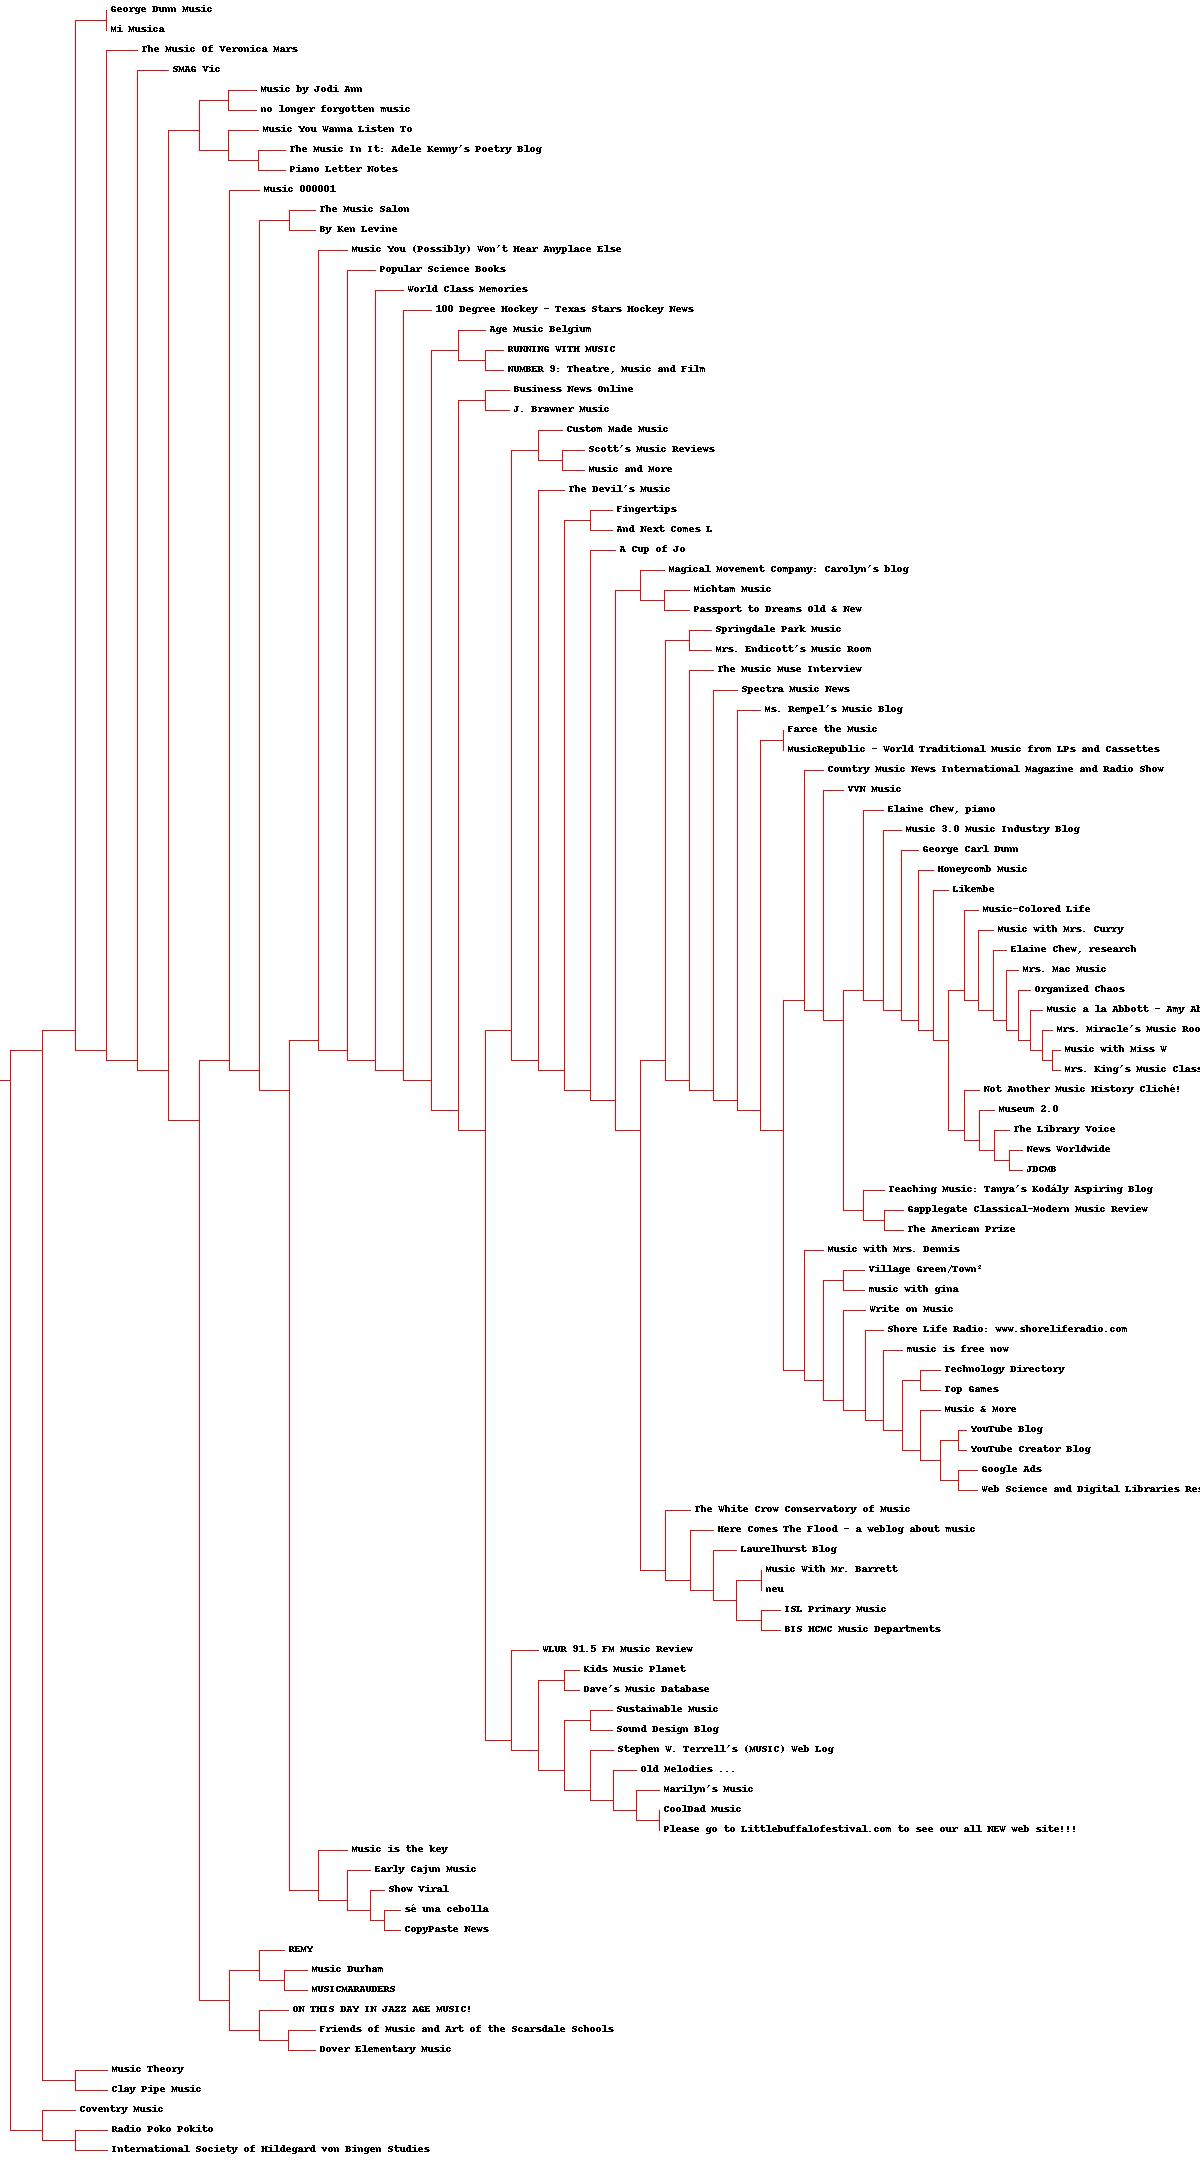
\includegraphics[width=.99\textwidth,height=.99\textheight]{../Figures/blogclust.jpg}%
        \caption{Dendogram}
    \end{figure}%
    \clearpage
}
\pagebreak

\section*{Question 3}

\subsection*{  Cluster the blogs using K-Means, using k=5,10,20.}

%------------------------------------------------
\bigskip\bigskip
\LARGE Solution: \newline\newline\small


\tabto{2.0cm} Using the kcluster function provided by the Programming Collective Intelligence book, K-Means of 5, 10, and 20 were calculated and recorded in the clusteredBlogs.txt file. In each case, a table is provided, displaying the clustered blogs in k groups. 

\begin{lstlisting}[language = Python, caption= Clustering into 5 groups]
kclust=clusters.kcluster(data,k=5)
kclust=clusters.kcluster(data,k=10)
kclust=clusters.kcluster(data,k=20)
\end{lstlisting}

\tabto{2.0cm} The code above returns a list indexed with a number of clusters, depending of the k value passed in. Using this function, the blogs are split into groups of five, ten, and twenty, and the data is accessed by the index of each group number as shown below.

\begin{lstlisting}[language = Python, caption= Clustering into 5 groups]
for x in range(0,5):

	for r in kclust[x]:
		centralFile.write(blognames[r] + '\n')
		centralFile.write('\n')
	centralFile.write('\n')
	centralFile.write("-------------------------------------------")
	centralFile.write('\n')
\end{lstlisting}


\begin{flushleft}
\begin{tabular}{ |p{2.8cm}||p{3.5cm}||p{2.8cm}||p{3cm}||p{3cm}|}
 \hline
 \multicolumn{5}{|c|}{Clustered Blogs in 5 Groups} \\
 \hline
 Cluster 1 & Cluster 2 & Cluster 3 & Cluster 4 & Cluster 5\\
 \hline
  Kids Music Planet & Music With Mr. Barrett & CoolDad Music & Farce the Music & A Cup of Jo  \\
  Music Theory & ISL Primary Music & George Dunn Music & Technology Directory & The Devil's Music\\
  Music and More & Top Games & Mrs. Mac Music & VVN Music & Michtam Music\\
  Age Music Belgium & Music with Miss W & News Worldwide & Clay Pipe Music & Custom Made Music\\
  Mi Musica & RUNNING WITH MUSIC & Music Durham & The Music Salon & Popular Science Books \\
 \hline
\end{tabular}
\end{flushleft}

\tabto{2.0cm} The table above contains blogs which were split into five clusters. The exact same procedure was followed to produce clusters of ten and twenty, which are contained within the ``clusteredBlogs.txt'' file. \newline \newline The number of iterations changes each time the program is run because the random k points may be located in different positions, and may thus be assigned different blogs. In this instance, the number of iterations required were 3 for k = 5, 5 for k = 10, and 6 for k = 20 

\pagebreak

\section*{Question 4}


\subsection*{Use MDS to create a JPEG of the blogs similar to slide 29 of the 
week 11 lecture.  How many iterations were required?}

%------------------------------------------------
\bigskip\bigskip
\LARGE Solution: \newline\newline\small

\tabto{2.0 cm} By passing the data list to the multidimensional scaling function provided by the Programming Collective Intelligence book, an image representing a two dimensional view of the distance between each blog is produced. This function attempts to move each node according to the combination of all the other nodes pushing and pulling on it, until the total amount of error cannot be reducted. In this case, it took 290 iterations until the amount of error had stabilized, and then the MDS was drawn.


 \begin{lstlisting}[language = Python, caption=Drawing 2d from Programming Collective Intelligence]
coords=clusters.scaledown(data)
clusters.draw2d(coords,blognames,jpeg='blogs2d.jpg')

\end{lstlisting}

\begin{figure}[p]%
        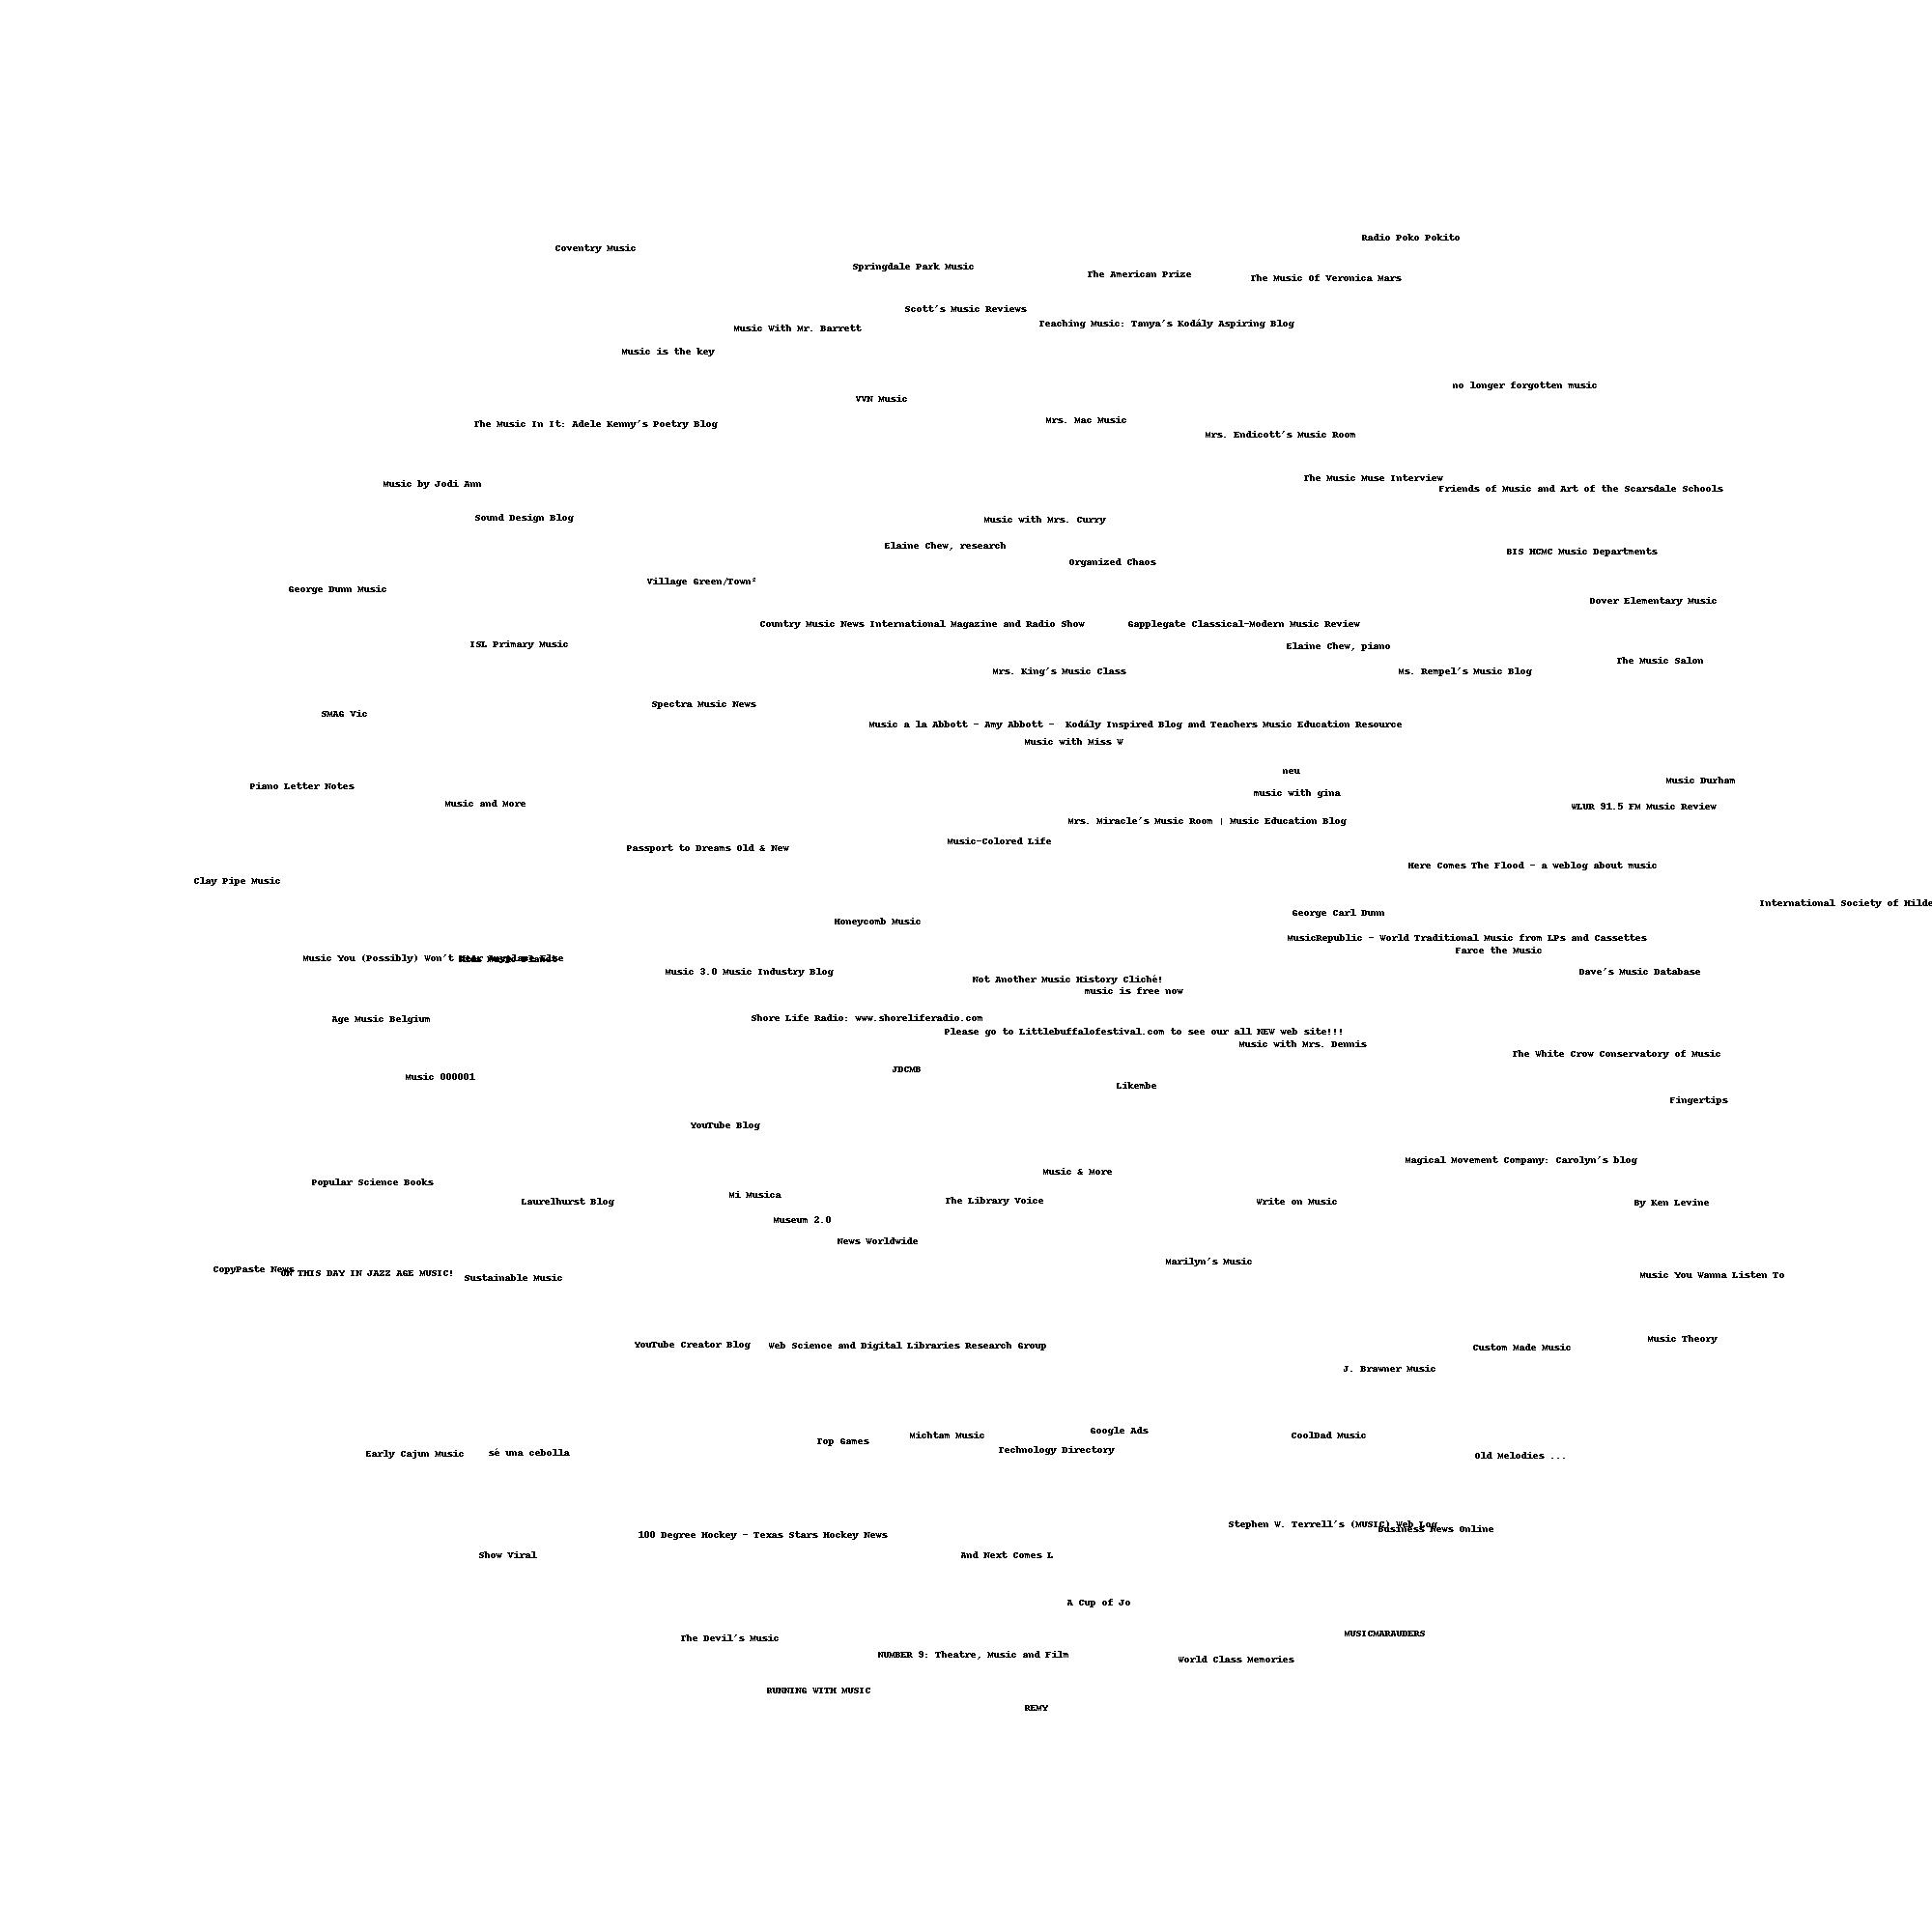
\includegraphics[width=.99\textwidth,height=.99\textheight]{../Figures/blogs2d.jpg}%
        \caption{2d Drawing}
    \end{figure}%

\bigskip \bigskip
\tabto{2.0cm} The image on the next page displays the 2d image created from the reduced nodes coordinates. These values appear to align with the general expectations. For example, ``Web Science and Digital Libraries'' appears near ``The Library Voice'', displaying a sense of relation between the two blogs.

\pagebreak
\section*{Question 6}


\subsection*{Re-run questions 1-4, but this time instead of using the 98 
"random" blogs, use 98 blogs that should be "similar" to:
http://f-measure.blogspot.com/
http://ws-dl.blogspot.com/}

\tabto{2.0cm} 98 other URIs were extracted by using Google and querying terms such as music, data science, data, and songs, among other terms. Using these URIs, the 2d figure, dendogram, and ASCII files were generated in the same manner as the original URIs. \newline \newline

\tabto{2.0cm} It is evident when comparing the dendograms and 2d files generated by the two data sets, that there are major differences. First and foremost, the ``similar'' dataset has increased structure and relations. For example, looking at the dendogram on page 10, it is evident that there is almost an entirely new branch with segments into data science. This branch does not exist in the original dendogram because there is a lack of URIs which relate to data science, therefore eleminating any possibility of the branch occurring. \newline \newline

\tabto{2.0cm} Moving on to the blogs2dExtraCredit, on page 11, it appears as though the clustering of related data has increased. For example, the ``Web Science and Digital Research Group'' is surronded by blogs such as ``Googld Ads'' and ``Technology Directory''. The same could be said for the 2dblog relating to the original URIs, but it is evident that, again, the new 2dblog file is more structured. Overall, the introduction of two distinct subjects exponentiates the differences in the terms, leading to more a more defined hierarchy, and thus a more defined structure.

\begin{figure}[p]%
        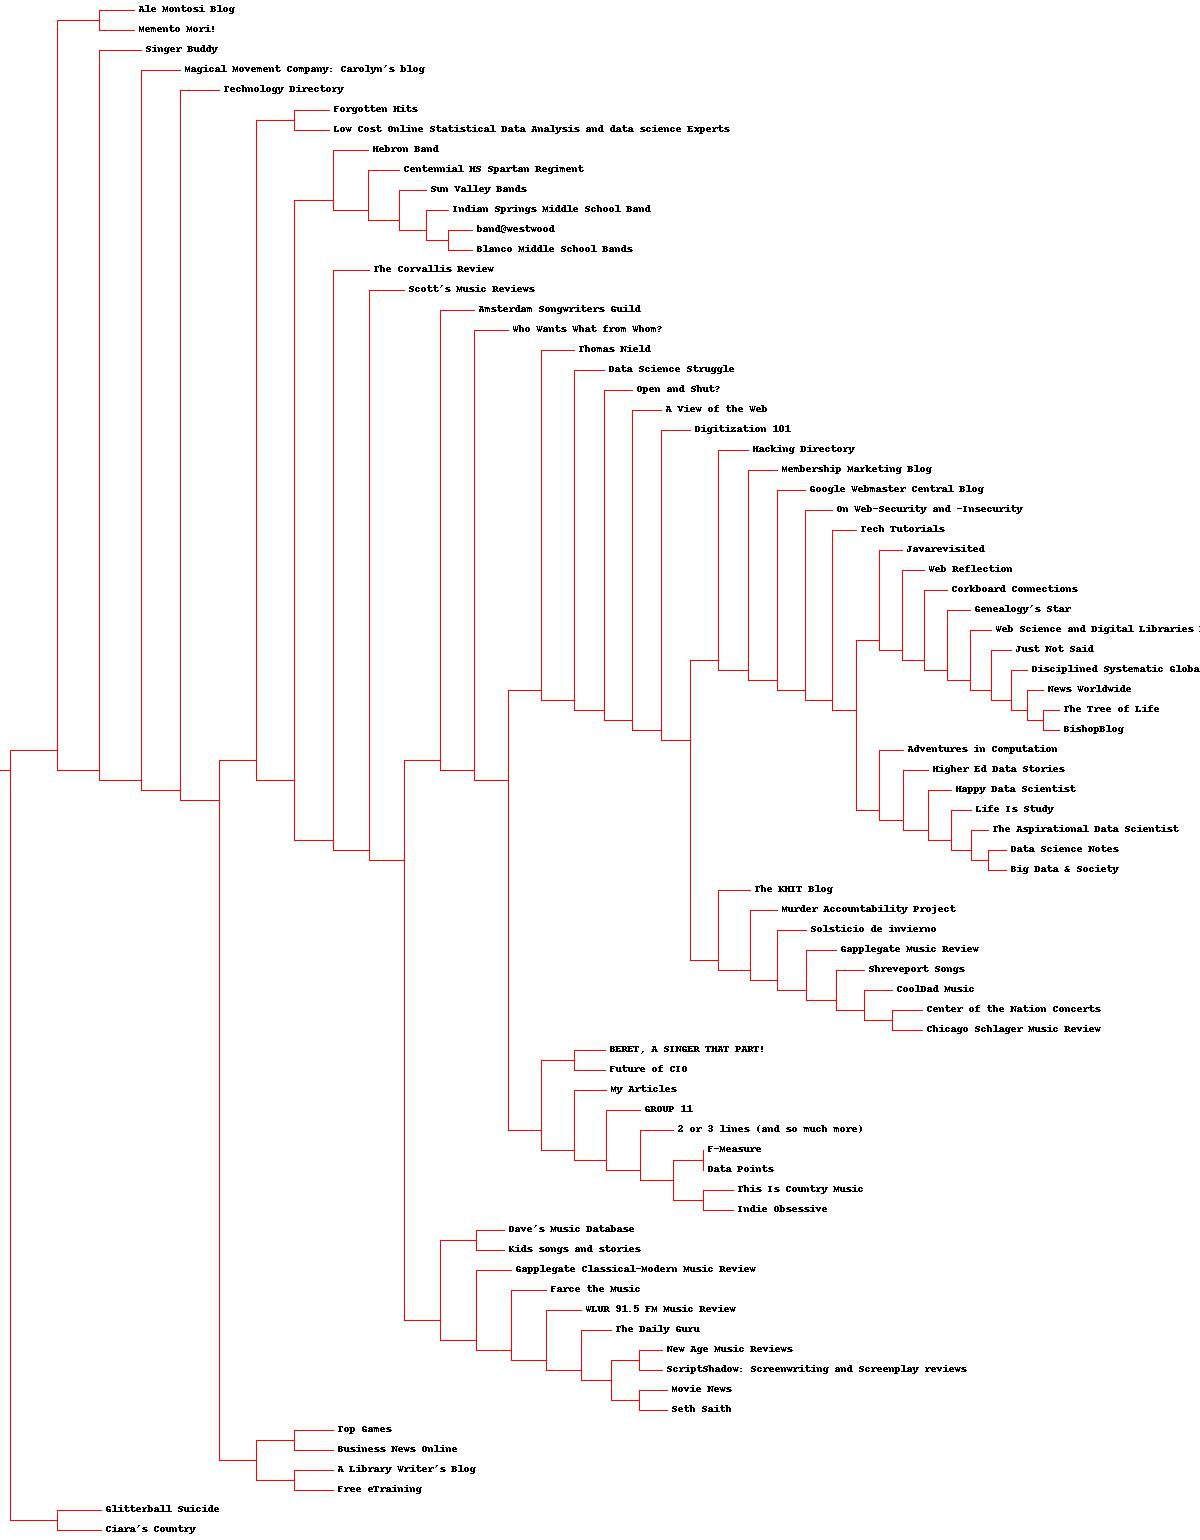
\includegraphics[width=.99\textwidth,height=.99\textheight]{../Figures/blogclustExtra.jpg}%
        \caption{Extra Credit Dendogram}
    \end{figure}%

    \begin{figure}[p]%
        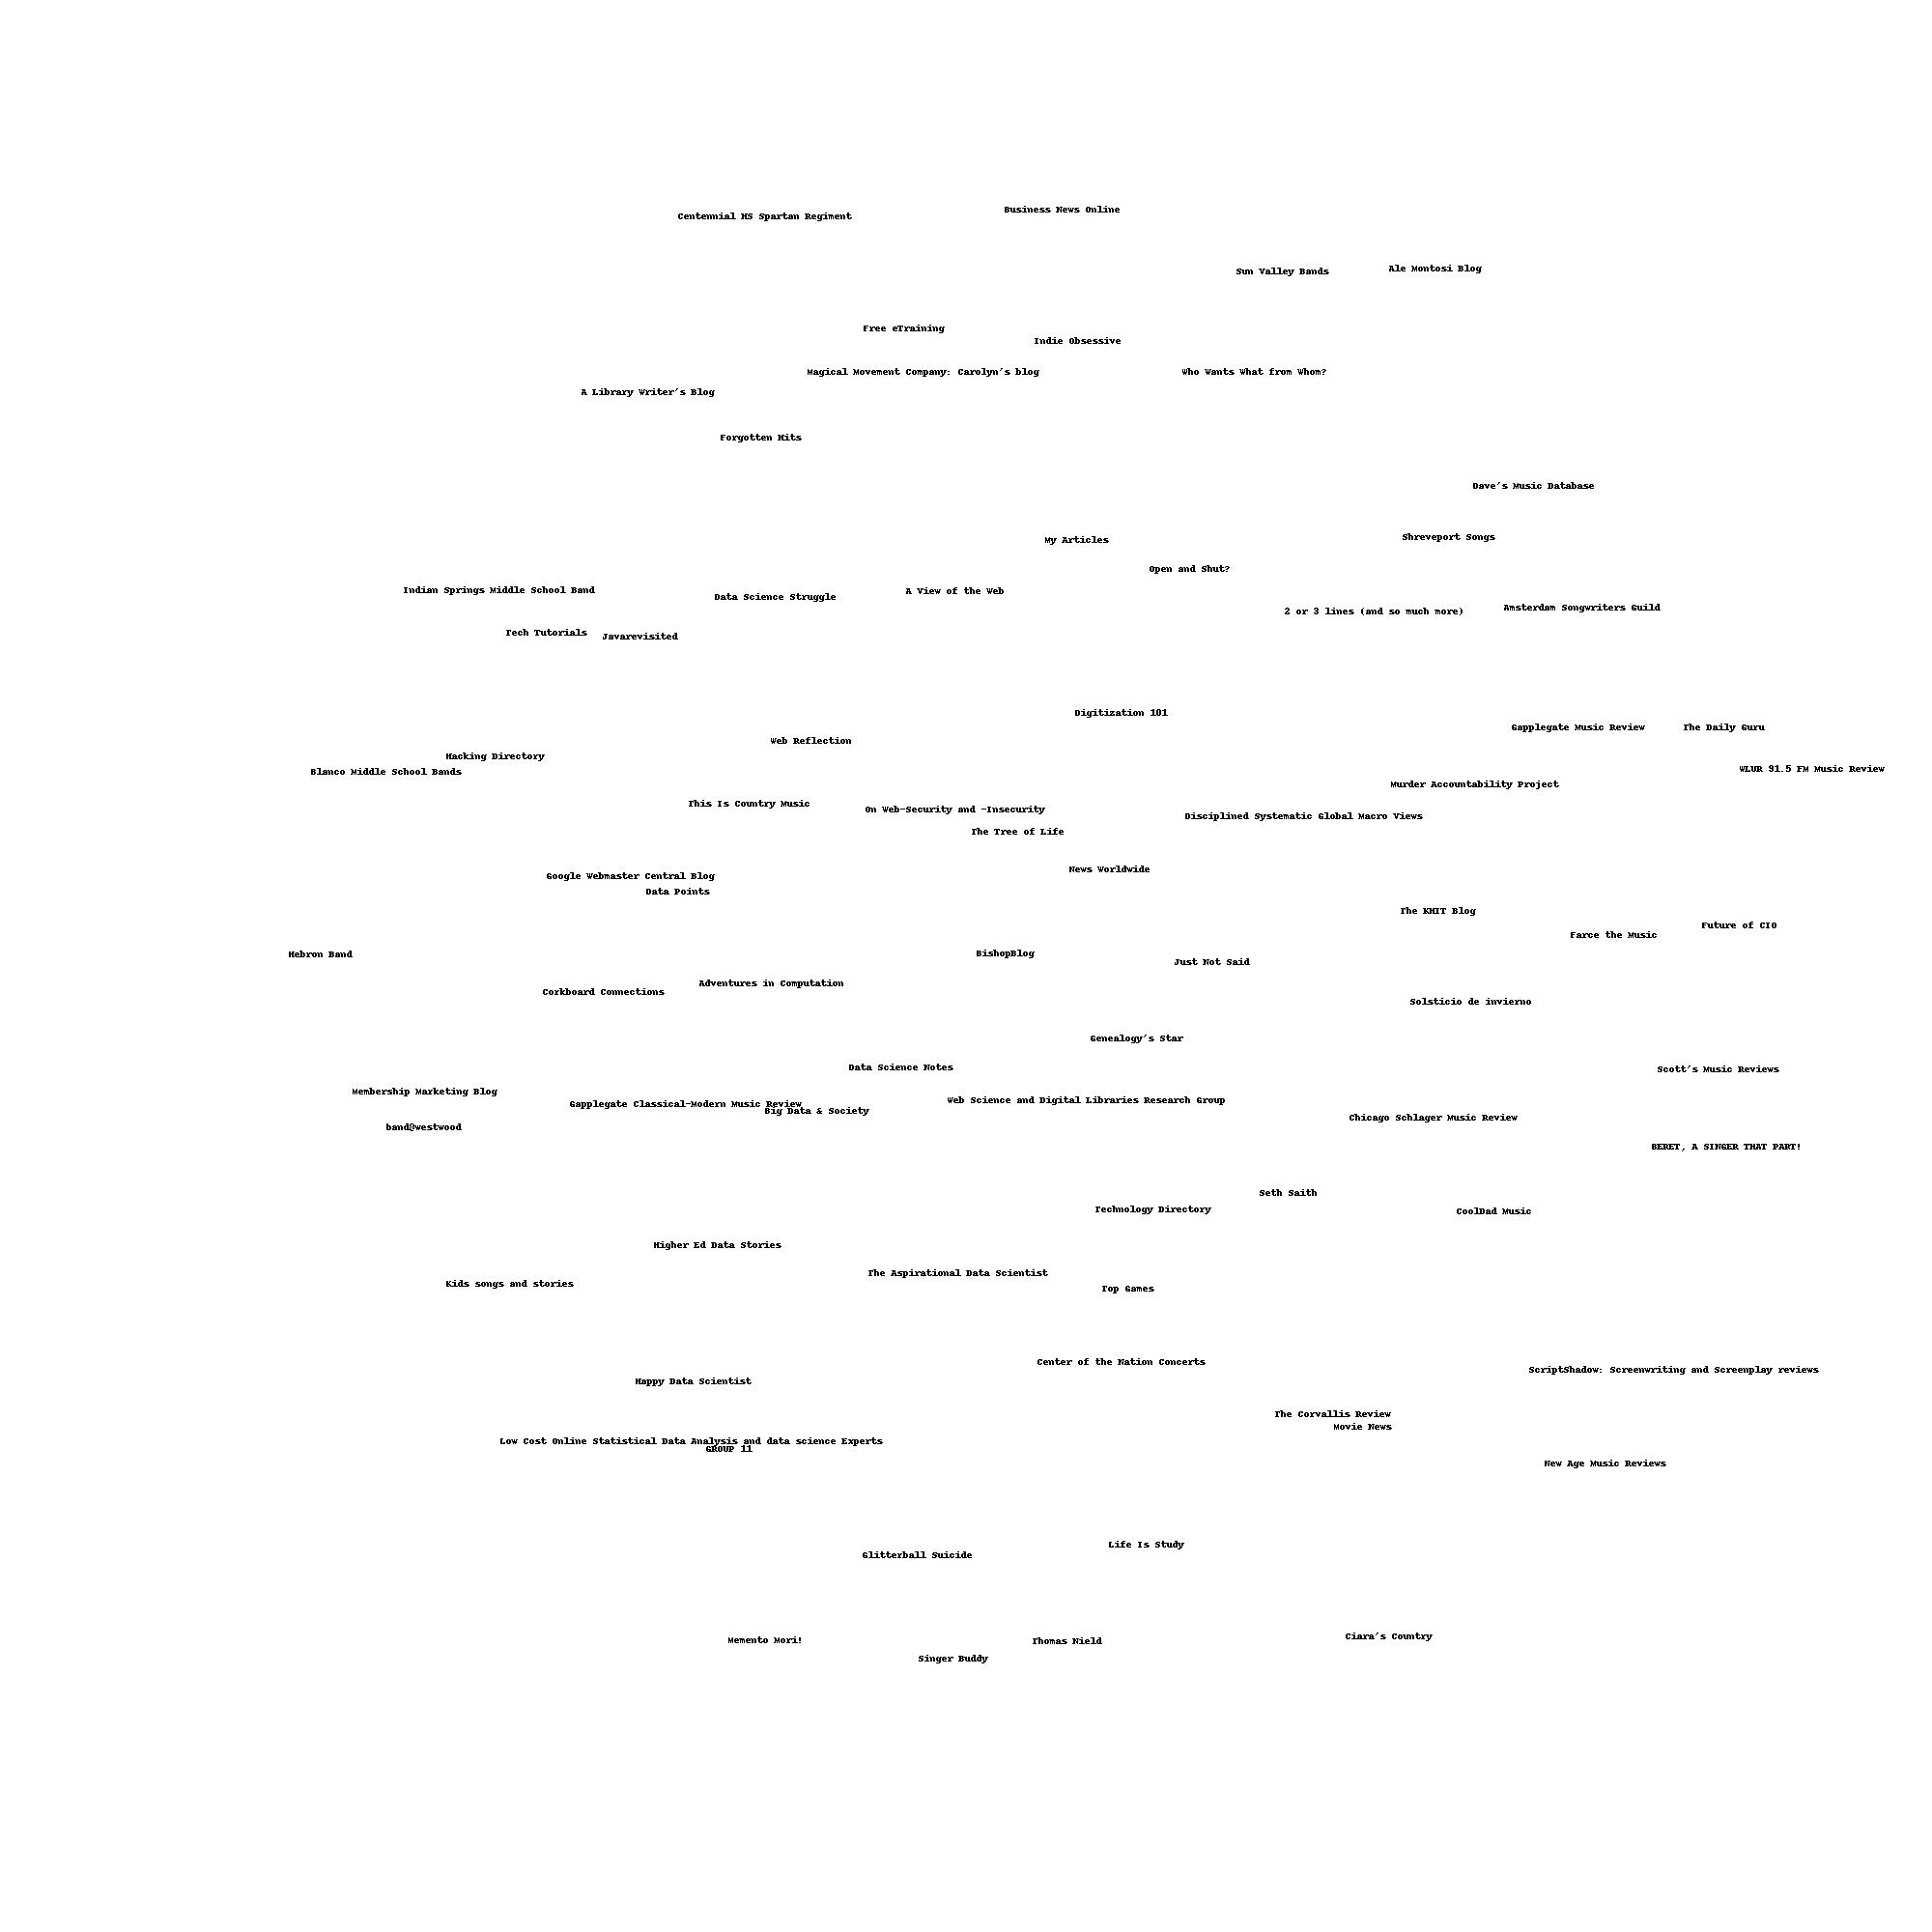
\includegraphics[width=.99\textwidth,height=.99\textheight]{../Figures/blogs2dExtra.jpg}%
        \caption{Extra Credit 2d Drawing}
    \end{figure}%



\end{document}
